% LuaLaTeX

\documentclass[a4paper, twoside, 12pt]{article}
\usepackage[latin]{babel}
%\usepackage[landscape, left=3cm, right=1.5cm, top=2cm, bottom=1cm]{geometry} % okraje stranky
%\usepackage[landscape, a4paper, mag=1166, truedimen, left=2cm, right=1.5cm, top=1.6cm, bottom=0.95cm]{geometry} % okraje stranky
\usepackage[landscape, a4paper, mag=1400, truedimen, left=0.5cm, right=0.5cm, top=0.5cm, bottom=0.5cm]{geometry} % okraje stranky

\usepackage{fontspec}
\setmainfont[FeatureFile={junicode.fea}, Ligatures={Common, TeX}, RawFeature=+fixi]{Junicode}
%\setmainfont{Junicode}

% shortcut for Junicode without ligatures (for the Czech texts)
\newfontfamily\nlfont[FeatureFile={junicode.fea}, Ligatures={Common, TeX}, RawFeature=+fixi]{Junicode}

\usepackage{multicol}
\usepackage{color}
\usepackage{lettrine}
\usepackage{fancyhdr}

% usual packages loading:
\usepackage{luatextra}
\usepackage{graphicx} % support the \includegraphics command and options
\usepackage{gregoriotex} % for gregorio score inclusion
\usepackage{gregoriosyms}
\usepackage{wrapfig} % figures wrapped by the text
\usepackage{parcolumns}
\usepackage[contents={},opacity=1,scale=1,color=black]{background}
\usepackage{tikzpagenodes}
\usepackage{calc}
\usepackage{longtable}
\usetikzlibrary{calc}

\setlength{\headheight}{14.5pt}

% Commands used to produce a typical "Conventus" booklet

\newenvironment{titulusOfficii}{\begin{center}}{\end{center}}
\newcommand{\dies}[1]{#1

}
\newcommand{\nomenFesti}[1]{\textbf{\Large #1}

}
\newcommand{\celebratio}[1]{#1

}

\newcommand{\hora}[1]{%
\vspace{0.5cm}{\large \textbf{#1}}

\fancyhead[LE]{\thepage\ / #1}
\fancyhead[RO]{#1 / \thepage}
\addcontentsline{toc}{subsection}{#1}
}

% larger unit than a hora
\newcommand{\divisio}[1]{%
\begin{center}
{\Large \textsc{#1}}
\end{center}
\fancyhead[CO,CE]{#1}
\addcontentsline{toc}{section}{#1}
}

% a part of a hora, larger than pars
\newcommand{\subhora}[1]{
\begin{center}
{\large \textit{#1}}
\end{center}
%\fancyhead[CO,CE]{#1}
\addcontentsline{toc}{subsubsection}{#1}
}

% rubricated inline text
\newcommand{\rubricatum}[1]{\textit{#1}}

% standalone rubric
\newcommand{\rubrica}[1]{\vspace{3mm}\rubricatum{#1}}

\newcommand{\notitia}[1]{\textcolor{red}{#1}}

\newcommand{\scriptura}[1]{\hfill \small\textit{#1}}

\newcommand{\translatioCantus}[1]{\vspace{1mm}%
{\noindent\footnotesize \nlfont{#1}}}

% pruznejsi varianta nasledujiciho - umoznuje nastavit sirku sloupce
% s prekladem
\newcommand{\psalmusEtTranslatioB}[3]{
  \vspace{0.5cm}
  \begin{parcolumns}[colwidths={2=#3}, nofirstindent=true]{2}
    \colchunk{
      \input{#1}
    }

    \colchunk{
      \vspace{-0.5cm}
      {\footnotesize \nlfont
        \input{#2}
      }
    }
  \end{parcolumns}
}

\newcommand{\psalmusEtTranslatio}[2]{
  \psalmusEtTranslatioB{#1}{#2}{8.5cm}
}


\newcommand{\canticumMagnificatEtTranslatio}[1]{
  \psalmusEtTranslatioB{#1}{temporalia/extra-adventum-vespers/magnificat-boh.tex}{12cm}
}
\newcommand{\canticumBenedictusEtTranslatio}[1]{
  \psalmusEtTranslatioB{#1}{temporalia/extra-adventum-laudes/benedictus-boh.tex}{10.5cm}
}

% volne misto nad antifonami, kam si zpevaci dokresli neumy
\newcommand{\hicSuntNeumae}{\vspace{0.5cm}}

% prepinani mista mezi notovymi osnovami: pro neumovane a neneumovane zpevy
\newcommand{\cantusCumNeumis}{
  \setgrefactor{17}
  \global\advance\grespaceabovelines by 5mm%
}
\newcommand{\cantusSineNeumas}{
  \setgrefactor{17}
  \global\advance\grespaceabovelines by -5mm%
}

% znaky k umisteni nad inicialu zpevu
\newcommand{\superInitialam}[1]{\gresetfirstlineaboveinitial{\small {\textbf{#1}}}{\small {\textbf{#1}}}}

% pars officii, i.e. "oratio", ...
\newcommand{\pars}[1]{\textbf{#1}}

\newenvironment{psalmus}{
  \setlength{\parindent}{0pt}
  \setlength{\parskip}{5pt}
}{
  \setlength{\parindent}{10pt}
  \setlength{\parskip}{10pt}
}

%%%% Prejmenovat na latinske:
\newcommand{\nadpisZalmu}[1]{
  \hspace{2cm}\textbf{#1}\vspace{2mm}%
  \nopagebreak%

}

% mode, score, translation
\newcommand{\antiphona}[3]{%
\hicSuntNeumae
\superInitialam{#1}
\includescore{#2}

#3
}
 % Often used macros
%%%% Preklady jednotlivych zpevu (nektere se opakuji, a je dobre mit je
% vsechny na jedne hromade)

\newcommand{\trOratioAnteOfficium}{\translatioCantus{Otevři, Pane, má ústa, abych chválil tvé svaté jméno.
Očisti mé srdce od všech marnivých, zvrácených a~jiných myšlenek, osvěť rozum, rozněť cit,
abych mohl důstojně, soustředěně a~zbožně recitovat a~vysloužil si být
vyslyšen před tváří tvé velebnosti. Skrze Krista…}}

\newcommand{\trOratioPostOfficium}{\translatioCantus{\textit{Následující modlitbu
opatřil pro ty, kdo ji zbožně vyřknou po hodinkách, zesnulý papež Lev X.
odpustky za hříchy vzniklé při konání hodinek z~lidské křehkosti. Říká se
vkleče.}
Svatosvaté a~nerozdílné Trojici, ukřižovanému lidství našeho Pána Ježíše
Krista, přeblažené a~přeslavné plodné neporušenosti vždy Panny Marie
i~souhrnu všech svatých buď ode všeho stvoření věčná chvála, čest a~sláva, nám
pak buď dáno odpuštění všech hříchů, po nekonečné věky věků. Amen.}}

% HOURS ---

\newcommand{\trAntI}{\translatioCantus{Jasné narození slavné Panny Marie,
z pokolení (dosl. ze semene) Abrahámova, vzešlé z kmene Judova, z rodu Davidova.}}
\newcommand{\trAntII}{\translatioCantus{Dnes je Narození svaté Panny 
Marie, jejíž předrahý život osvěcuje všechny církve.}}

\newcommand{\trAntIII}{\translatioCantus{Maria, jež vzešla 
z královského rodu, září; myslí i duchem ji zbožně prosíme, aby 
nám pomáhala svými přímluvami.}}

\newcommand{\trAntIV}{\translatioCantus{Srdcem i duchem pějme Kristu 
k slávě o této svaté slavnosti vznešené Rodičky Boží Marie.}}

\newcommand{\trAntV}{\translatioCantus{Příjemně \notitia{?} 
oslavujme Narození blahoslavené Marie,
aby se ona za nás přimlouvala u Pána Ježíše Krista.}}

\newcommand{\trCapituli}{\translatioCantus{Před věky, na počátku mě stvořil, potrvám věčně. Ve svatém Stanu jsem před ním konala službu.}}

\newcommand{\trRespVesp}{\translatioCantus{Buď zdráva, Maria,
plná milosti: \grestar{} Pán s tebou. \Vbardot{} Požehnaná jsi mezi ženami,
a požehnaný plod života (ve smyslu lůna, břicha) tvého.}}

\newcommand{\trVersus}{\translatioCantus{\Vbardot{} Dnes je Narození svaté Panny Marie. \Rbardot{} Jejíž předrahý život osvěcuje všechny církve.}}

\newcommand{\trAntMagnificatI}{\translatioCantus{Konejme památku
veledůstojného narození slavné Panny Marie,
jíž se dostalo mateřské důstojnosti bez ztráty panenské cudnosti.}}

% Tento preklad je vice nez nejisty a ani alternativy, ktere jsem
% videl, me nepresvedcily...
\newcommand{\trAntBenedictus}{\translatioCantus{Slavnostně slavme 
dnešní narození Marie, vždy Panny a Rodičky Boží: v něm se objevuje
vysokost trůnu (totiž Marie, trůnu Božího Syna), aleluja.}}

\newcommand{\trAntMagnificatII}{\translatioCantus{Tvé narození,
Bohorodičko Panno, vyhlásilo radost celému světu:
z tebe totiž vzešlo Slunce spravedlnosti, Kristus, náš Bůh:
jenž zrušil kletbu a dal nám požehnání: přemohl smrt a dal nám život věčný.}}

\newcommand{\trOrationis}{\translatioCantus{Prosíme tě, Bože, 
uděl svým služebníkům dar nebeské milosti,
aby těm, jimž slehnutím blahoslavené Panny vyvstal počátek spásy, 
slavnost k poctě jejího narození přinesla
rozhojnění pokoje.
Skrze tvého Syna, našeho Pána Ježíše Krista, který s tebou žije a kraluje,
Bůh, v jednotě Ducha svatého po všechny věky věků.}}

\newcommand{\trFideliumAnimae}{\translatioCantus{\Vbardot{} Duše věrných ať pro
milosrdenství Boží odpočívají v~pokoji. \Rbardot{} Amen.}}

% Completorium

\newcommand{\trJubeDomne}{\translatioCantus{Rač, pane, požehnat.}}

\newcommand{\trComplBenedictio}{\translatioCantus{Pokojnou noc a~svatou smrt
nechť nám dopřeje všemohoucí Pán. \Rbardot{} Amen.}}

\newcommand{\trComplLectioBr}{\translatioCantus{Buďte střízliví, bděte.
Váš protivník Ďábel obchází jako lev řvoucí a~hledá, koho by pohltil.
Postavte se proti němu pevní ve víře.  Ale ty, Pane, smiluj se nad námi.
\Rbardot{} Bohu díky.}}

\newcommand{\trComplAntI}{\translatioCantus{Rač se smilovati nade mnou,
Hospodine, a vyslyš mou modlitbu.}}

\newcommand{\trComplCapituli}{\translatioCantus{Jsi přece, Hospodine,
uprostřed nás a~jmenujeme se po tobě.  Neopouštěj nás, Pane, náš Bože.}}

\newcommand{\trRespCompl}{\translatioCantus{Do tvých rukou, Pane, \grestar{}
poroučím svého ducha. \Vbardot{} Ty mne zachráníš, Pane, Bože věrný.}}

\newcommand{\trComplVersus}{\translatioCantus{\Vbardot{} Střez mne jako zřítelnici oka,
aleluja. \Rbardot{} Ve stínu svých křídel uschovej mne, aleluja.}}

\newcommand{\trAntSalvaNos}{\translatioCantus{Ochraňuj nás, Pane, když
bdíme, a~buď s~námi, když spíme, ať bdíme s~Kristem a~odpočíváme v~pokoji.}}

\newcommand{\trComplOrationis}{\translatioCantus{Zavítej, prosíme, Pane, sem
do našeho příbytku a~daleko od něj zažeň všechny úklady nepřítele. Ať tu
bydlí tví svatí andělé a~tvoje požehnání buď nad ním stále. Skrze…}}

\newcommand{\trSalveRegina}{\translatioCantus{Zdrávas Královno, matko
milosrdenství, živote, sladkosti a naděje naše, buď zdráva!
K tobě voláme, vyhnaní synové Evy,
k tobě vzdycháme, lkajíce a plačíce
v tomto slzavém údolí.
A proto, orodovnice naše,
obrať k nám své milosrdné oči
a Ježíše, požehnaný plod života svého,
nám po tomto putování ukaž,
ó milostivá, ó přívětivá,
ó přesladká, Panno Maria!}}

\newcommand{\trOraProNobis}{\translatioCantus{\Vbardot{} 
Oroduj za nás, svatá Boží Rodičko,
\Rbardot{} aby nám Kristus dal účast na svých zaslíbeních.}}

% Matutinum

\newcommand{\trMatInvitatorium}{\translatioCantus{}}

\newcommand{\trMatVeniteA}{\translatioCantus{Pojďte, chvalme s~radostí Pána,
s~jásotem slavme Boha, svou spásu; předstupme před tvář jeho s~díky, písně plesu pějme jemu.}}

\newcommand{\trMatVeniteB}{\translatioCantus{Neboť Bůh veliký jest Hospodin, a~král nade všecky bohy.
Jsouť v~jeho ruce všecky hlubiny země, temena hor jsou majetek jeho.}}

\newcommand{\trMatVeniteC}{\translatioCantus{Jehoť jest moře, neb on je učinil; i~souš
je dílo jeho rukou. Pojďme, klanějme se, padněme, klekněme před Pánem, svým
tvůrcem. Jeť on Pán, náš Bůh, a~my jsme lid, jejž on vodí a~ovce, jež pase.}}

\newcommand{\trMatVeniteD}{\translatioCantus{Kéž byste poslechli dnes hlasu jeho:
,,Nezatvrzujte svých srdcí jak v~Hádce, jak v~Pokušení na poušti, kde vaši otcové pokoušeli mne,
zkoušeli mne, ač vídali skutky mé.``}}

\newcommand{\trMatVeniteE}{\translatioCantus{Čtyřicet roků mrzel jsem se na to pokolení
a~řekl jsem: ,,Lid je to myslí stále bloudící``! Oni však nechtěli znáti mé cesty, takže jsem
přisáhl ve svém hněvu: ,,Nedojdou odpočinku mého!\mbox{}``}}

\newcommand{\trMatAntI}{\translatioCantus{}}

\newcommand{\trMatAntII}{\translatioCantus{}}

\newcommand{\trMatAntIII}{\translatioCantus{}}

\newcommand{\trMatVersusI}{\translatioCantus{}}

\newcommand{\trMatAbsolutioI}{\translatioCantus{Vyslyš Pane Ježíši Kriste
prosby svých služebníků \gredagger{} a~smiluj se nad námi, \grestar{} jenž
s~Otcem a~Duchem…}}

\newcommand{\trMatBenedictioI}{\translatioCantus{Rač, pane, požehnat.
Věčný Otec nám stále žehnej. \Rbardot{} Amen.}}

\newcommand{\trMatLecI}{\translatioCantus{Kéž by mě zulíbal polibky svých úst. 
Tvé milování je nad víno lahodnější;
vybraně voní tvé voňavky;
rozlévající se olej je tvé jméno,
proto tě dívky milují.
Strhni mě za sebou, poběžme!
Král mě uvedl do svých komnat;
budeš nám radostí a jásotem.
Víc než víno oslavíme tvé milování;
věru po právu jsi milován!
Snědá jsem, a přece krásná, jeruzalémské dcery,
jako stany kedarské,
jako šalmské závěsy.
}}

\newcommand{\trMatRespI}{\translatioCantus{}}

\newcommand{\trMatBenedictioII}{\translatioCantus{Rač, pane, požehnat.
Jednorozený Boží Syn nám žehnej \grestar{} a nám pomáhej. \Rbardot{} Amen.}}

\newcommand{\trMatLecII}{\translatioCantus{Nehleďte na mou osmahlou pleť:
to mě slunce ožehlo.
Synové mé matky se na mne rozzlobili,
poslali mě hlídat vinice.
A svou vinici, tu jsem nehlídala!
Pověz mi tedy, ty, jehož miluje mé srdce:
kam zavedeš své stádo pást,
kde ho necháš za poledne odpočívat?
Abych už nebloudila jako tulačka
poblíž stád druhů tvých.
Nevíš-li to, nejrásnější z žen,
jdi po stopách stáda
a kůzlata svá zaveď, ať se pasou
poblíž obydlí pastýřů.
Ke své klisně zapřažené do vozu faraonova
tebe, mé milá, přirovnávám.
Stále krásné jsou tvé líce s náušnicemi
i tvé hrdlo v náhrdelnících.}}

\newcommand{\trMatRespII}{\translatioCantus{}}

\newcommand{\trMatBenedictioIII}{\translatioCantus{Rač, pane, požehnat.
Milost Ducha Svatého ať osvítí nám smysly \grestar{} i srdce. \Rbardot{} Amen.}}

\newcommand{\trMatLecIII}{\translatioCantus{Zhotovíme ti zlaté náušnice
a kuličky ze stříbra.
Když král stoluje,
vydechuje můj nard svou vůni.
Můj milý je polštářek s myrhou,
jenž mi odpočívá mezi ňadry.
Můj milý je hrozen šáchoru
ve vinicích v Engadi.
Jak jsi krásná, milá moje,
jak jsi krásná!
Tvé oči jsou holubice.
Jak jsi krásný, můj milý,
jak líbezný!
Naše lože je samá zeleň.
Trámoví našeho domu je z cedru,
naše ostění z cypřiše.}}

\newcommand{\trMatRespIII}{\translatioCantus{}}

\newcommand{\trMatAntIV}{\translatioCantus{}}

\newcommand{\trMatAntV}{\translatioCantus{}}

\newcommand{\trMatAntVI}{\translatioCantus{}}

\newcommand{\trMatVersusII}{\translatioCantus{}}

\newcommand{\trMatAbsolutioII}{\translatioCantus{
Tvá milost a laskavost nechť nám pomáhá, jenž žiješ a vládneš s Otcem a Svatým Duchem na věky věků.}}

\newcommand{\trMatBenedictioIV}{\translatioCantus{Rač, pane, požehnat.
Bůh Otec všemohoucí, \grestar{} buď k nám milostivý a odpouštějící. \Rbardot{} Amen.}}

\newcommand{\trMatLecIV}{\translatioCantus{}}

\newcommand{\trMatRespIV}{\translatioCantus{}}

\newcommand{\trMatBenedictioV}{\translatioCantus{}}

\newcommand{\trMatLecV}{\translatioCantus{}}

\newcommand{\trMatRespV}{\translatioCantus{}}

\newcommand{\trMatBenedictioVI}{\translatioCantus{Rač, pane, požehnat.
Bůh rozněť v nás oheň své lásky. \Rbardot{} Amen.}}

\newcommand{\trMatLecVI}{\translatioCantus{}}

\newcommand{\trMatRespVI}{\translatioCantus{}}

\newcommand{\trMatAntVII}{\translatioCantus{}}

\newcommand{\trMatAntVIII}{\translatioCantus{}}

\newcommand{\trMatAntIX}{\translatioCantus{}}

\newcommand{\trMatVersusIII}{\translatioCantus{}}

\newcommand{\trMatAbsolutioIII}{\translatioCantus{Z okovů našich hříchů,
\grestar{} vysvoboď nás všemohoucí a milosrdný Pán. \Rbardot{} Amen.}}

\newcommand{\trMatBenedictioVII}{\translatioCantus{Rač, pane, požehnat.
Čtení evangelia nechť je nám \grestar{} spásou a ochranou. \Rbardot{} Amen.}}

\newcommand{\trMatLecVIIa}{\translatioCantus{
  Rodokmen Ježíše Krista, syna Davidova, syna Abrahámova:
  Abrahám zplodil Izáka,
  Izák zplodil Jakuba.}}

\newcommand{\trMatLecVIIb}{\translatioCantus{}}

\newcommand{\trMatRespVII}{\translatioCantus{}}

\newcommand{\trMatBenedictioVIII}{\translatioCantus{Rač, pane, požehnat.
\Rbardot{} Amen.}}

\newcommand{\trMatLecVIII}{\translatioCantus{}}

\newcommand{\trMatRespVIII}{\translatioCantus{}}

\newcommand{\trMatBenedictioIX}{\translatioCantus{Rač, pane, požehnat.
Do společnosti občanů nebes \grestar{} ať nás dovede král andělů.
\Rbardot{} Amen.}}

\newcommand{\trMatLecIX}{\translatioCantus{}}

% from the Czech Liturgia horarum
\newcommand{\trTeDeum}{\begin{translatioMulticol}{3}

Bože, tebe chválíme, 
tebe, Pane, velebíme.

Tebe, věčný Otče, 
oslavuje celá země.

Všichni andělé, 
cherubové i~serafové,

všechny mocné nebeské zástupy 
bez ustání volají:

Svatý, Svatý, Svatý, 
Pán, Bůh zástupů.

Plná jsou nebesa i~země 
tvé vznešené slávy.

Oslavuje tě 
sbor tvých apoštolů,

chválí tě 
velký počet proroků,

vydává o~tobě svědectví 
zástup mučedníků;

a~po celém světě 
vyznává tě tvá církev:

neskonale velebný, 
všemohoucí Otče,

úctyhodný Synu Boží, 
pravý a~jediný,

božský Utěšiteli, 
Duchu svatý.

Kriste, Králi slávy, 
tys od věků Syn Boha Otce;

abys člověka vykoupil, 
stal ses člověkem a~narodil ses z~Panny;

zlomil jsi osten smrti 
a~otevřel věřícím nebe;

sedíš po Otcově pravici 
a~máš účast na jeho slávě.

Věříme, že přijdeš soudit, 

a~proto tě prosíme:
přispěj na pomoc svým služebníkům, 
vždyť jsi je vykoupil svou předrahou krví;

dej, ať se radují s~tvými svatými 
ve věčné slávě.

Zachraň, Pane, svůj lid, žehnej svému dědictví, 
veď ho a~stále pozvedej.

Každý den tě budeme velebit 
a~chválit tvé jméno po všechny věky.

Pomáhej nám i~dnes, 
ať se nedostaneme do područí hříchu.

Smiluj se nad námi, Pane, 
smiluj se nad námi.

Ať spočine na nás tvé milosrdenství, 
jak doufáme v~tebe.

Pane, k~tobě se utíkáme, 
ať nejsme zahanbeni na věky. 
\end{translatioMulticol}}

\newcommand{\trMatEvangelium}{\translatioCantus{
  Rodokmen Ježíše Krista, syna Davidova, syna Abrahámova:
  Abrahám zplodil Izáka,
  Izák zplodil Jakuba,
  Jakub zplodil Judu a jeho bratry,
  Juda zplodil Farese a Zaru z Tamary,
  Fares zplodil Esroma,
  Esrom zplodil Arama,
  Aram zplodil Aminadaba,
  Aminadab zplodil Naasona,
  Naason zplodil Salmona,
  Salmon zplodil Boaze z Rahaby,
  Boaz zplodil Jobeda z Rut,
  Jobed zplodil Jessea,
  Jesse zplodil krále Davida.
  David zplodil Šalomouna z Uriášovy ženy,
  Šalomoun zplodil Roboama,
  Roboam zplodil Abiu,
  Abia zplodil Asu,
  Asa zplodil Josafata,
  Josafat zplodil Jorama,
  Joram zplodil Oziáše,
  Oziáš zplodil Joatama,
  Joatam zplodil Achaze,
  Achaz zplodil Ezechiáše,
  Ezechiáš zplodil Manasesa,
  Manases zplodil Amona,
  Amon zplodil Josiáše,
  Josiáš zplodil Jechoniáše a jeho bratry;
  tehdy došlo k odvlečení do Babylonu.
  Po odvlečení do Babylonu:
  Jechoniáš zplodil Salatiela,
  Salatiel zplodil Zorobabela,
  Zorobabel zplodil Abiuda,
  Abiud zplodil Eljakima,
  Eljakim zplodil Azora,
  Ator zplodil Sadoka,
  Sadok zplodil Achima,
  Achim zplodil Eliuda,
  Eliud zplodil Eleazara,
  Eleatar zplodil Matana,
  Matan zplodil Jakuba,
  Jakub zplodil Josefa, manžela Marie,
  z níž se narodil Ježíš, který se nazývá Kristus.}}

\newcommand{\trTeDecetLaus}{\translatioCantus{Tobě chvála, Tobě zpěvy, Tobě
sláva, Bohu Otci i~Synu i~Svatému Duchu, na věky věků. \Rbardot{} Amen.}}

% MASS ---

\newcommand{\trIntroitus}{\translatioCantus{Radujme se všichni
v Pánu, slavíce svátek ke cti Panny Marie: z něj se radují andělé
a spoluchválí Božího Syna. \textit{\color{red}Žl.} Má ústa vydala dobré slovo,
přednáším svá díla králi.}}

\newcommand{\trGraduale}{\translatioCantus{Požehnaná a ctihodná jsi,
Panno Maria: nedotčená (co do panenství) jsi byla shledána matkou
Spasitele. \Vbardot{} Panno Boží Rodičko, ten, jehož nepojme ani celý svět,
se uzavřel do tvých útrob, když se stal člověkem.}}

\newcommand{\trAlleluia}{\translatioCantus{Aleluja. \Vbardot{} Skvělá slavnost
slavné Panny Marie, z pokolení (dosl. ze semene) Abrahámova, vzešlé z kmene 
Judova, z rodu Davidova.}}

\newcommand{\trOffertorium}{\translatioCantus{Blažená jsi, Panno Maria,
tys nosila Stvořitele všeho; porodila jsi toho, který tě utvořil,
a na věky zůstáváš Pannou.}}

\newcommand{\trCommunio}{\translatioCantus{Budou mě blahoslavit
všechna pokolení, protože mi učinil veliké věci ten, který je mocný.}}

% LITTLE HOURS ---

\newcommand{\trVersusTertia}{\translatioCantus{\Vbardot{} \Rbardot{}}}

\newcommand{\trCapituliEtSic}{\translatioCantus{
Tak jsem se usadila na Sionu a v milovaném městě jsem nalezla odpočinek,
v Jeruzalémě vykonávám svou moc.
Zakořenila jsem u lidu plného slývy, na panství Páně, v jeho dědictví.}}

\newcommand{\trVersusSexta}{\translatioCantus{\Vbardot{} \Rbardot{}}}

\newcommand{\trCapituliInPlateis}{\translatioCantus{
Na planině jako skořicovník a akant jsem vydávala vůni, jako vybraná myrha
jsem voněla.}}

\newcommand{\trVersusNona}{\translatioCantus{\Vbardot{} \Rbardot{}}}
 % Czech translations of the proper texts

\newcommand{\annusEditionis}{2020}

%%%% Vicekrat opakovane kousky

\newcommand{\anteOrationem}{
  \rubrica{Ante Orationem, cantatur a Superiore:}

  \pars{Supplicatio Litaniæ.}

  \cuminitiali{}{temporalia/supplicatiolitaniae.gtex}

  \pars{Oratio Dominica.}

  \cuminitiali{}{temporalia/oratiodominica.gtex}

  \rubrica{Deinde dicitur ab Hebdomadario:}

  \cuminitiali{}{temporalia/dominusvobiscum-solemnis.gtex}

  \rubrica{In choro monialium loco Dominus vobiscum dicitur:}

  \sineinitiali{temporalia/domineexaudi.gtex}
}

\setlength{\columnsep}{30pt} % prostor mezi sloupci

%%%%%%%%%%%%%%%%%%%%%%%%%%%%%%%%%%%%%%%%%%%%%%%%%%%%%%%%%%%%%%%%%%%%%%%%%%%%%%%%%%%%%%%%%%%%%%%%%%%%%%%%%%%%%
\begin{document}

% Here we set the space around the initial.
% Please report to http://home.gna.org/gregorio/gregoriotex/details for more details and options
\grechangedim{afterinitialshift}{2.2mm}{scalable}
\grechangedim{beforeinitialshift}{2.2mm}{scalable}
\grechangedim{interwordspacetext}{0.22 cm plus 0.15 cm minus 0.05 cm}{scalable}%
\grechangedim{annotationraise}{-0.2cm}{scalable}

% Here we set the initial font. Change 38 if you want a bigger initial.
% Emit the initials in red.
\grechangestyle{initial}{\color{red}\fontsize{38}{38}\selectfont}

\pagestyle{empty}

%%%% Titulni stranka
\begin{titulusOfficii}
\dies{Die 1. Novembris.}
\nomenFesti{In Festo Omnium Sanctorum.}
\celebratio{Duplex I. classis.}
\end{titulusOfficii}

% graphic
%\vspace{1.5cm}
%\begin{center}
%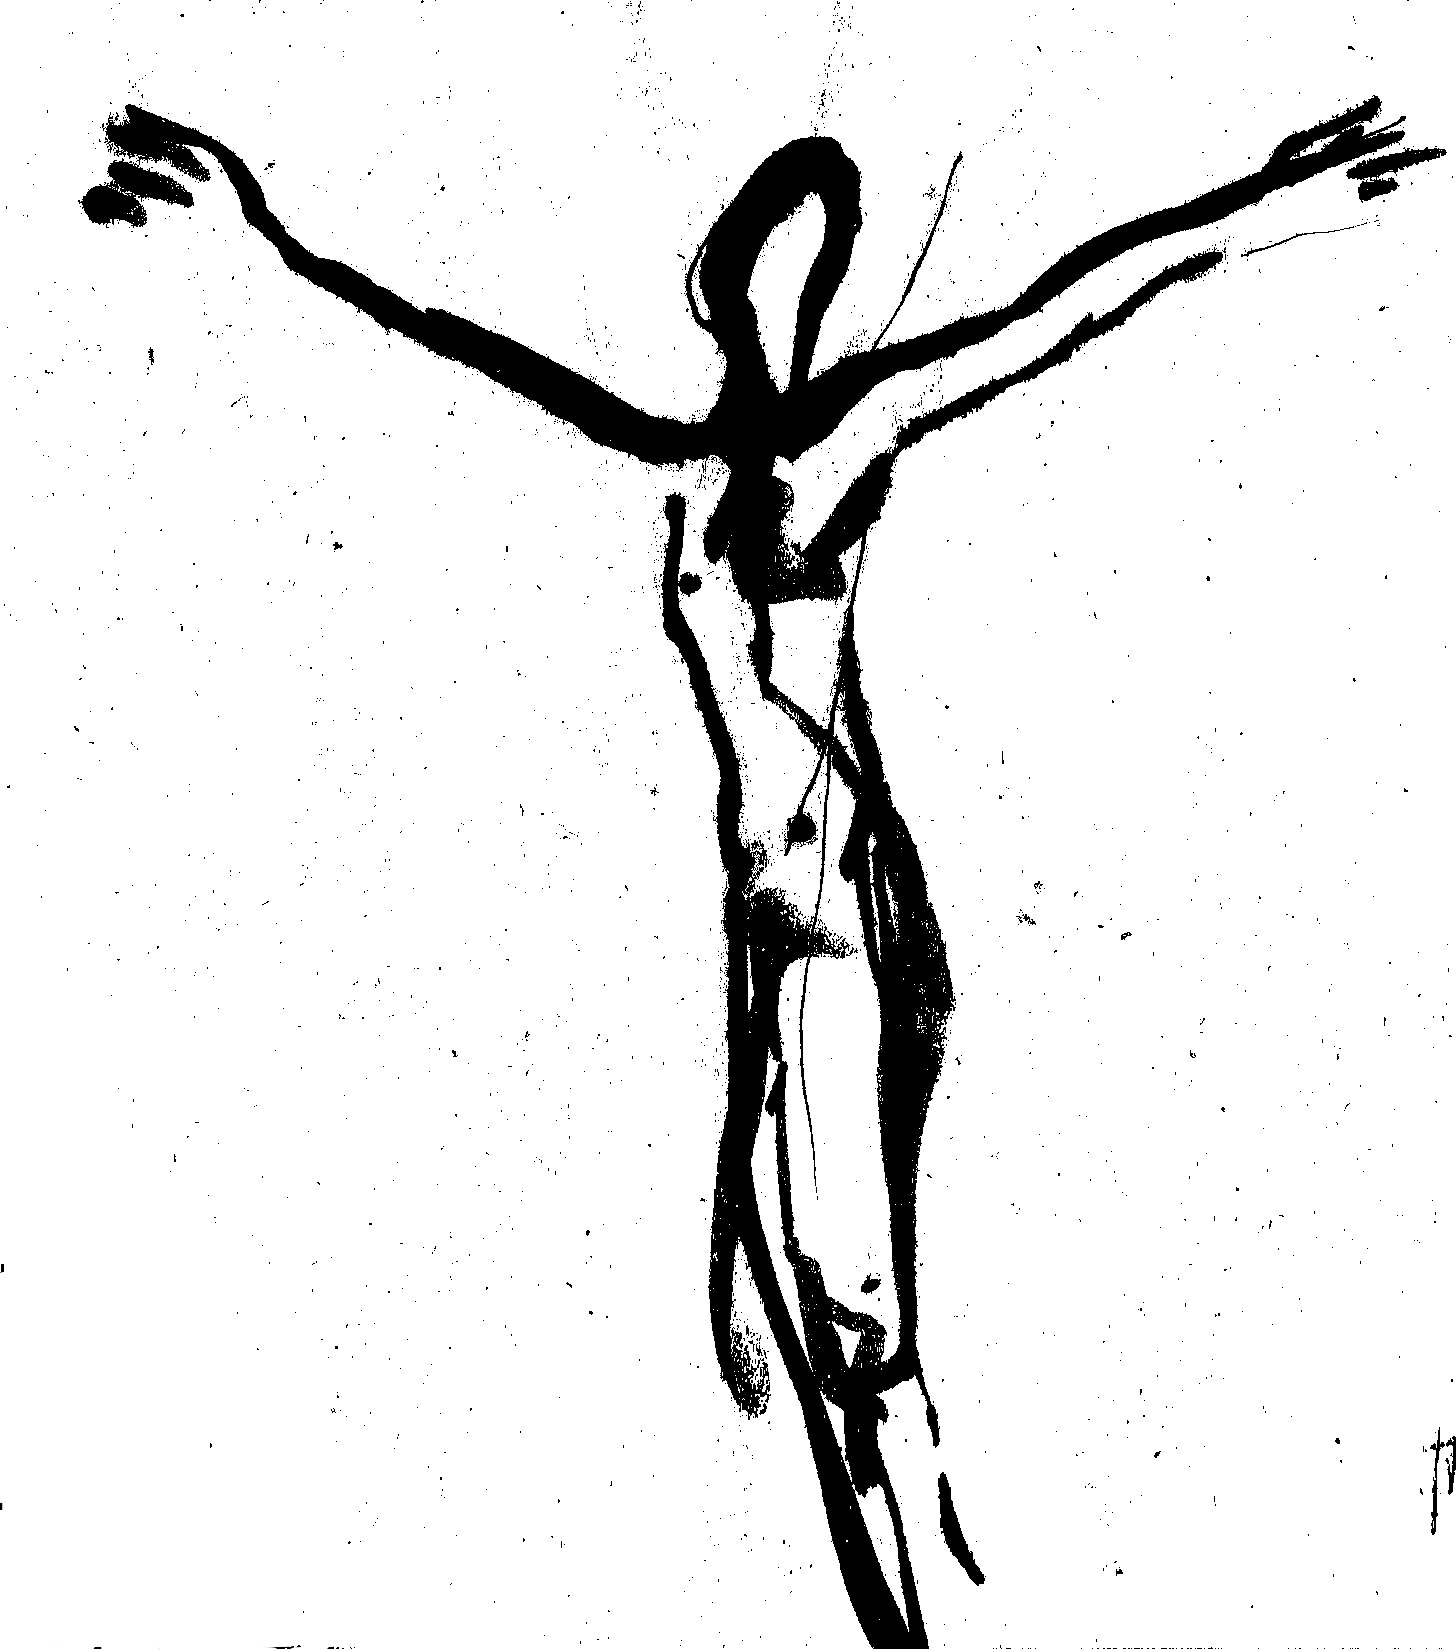
\includegraphics[height=8cm]{crux.jpg}
%\end{center}

\vfill

\begin{center}
%Ad usum et secundum consuetudines chori \guillemotright{}Conventus Choralis\guillemotleft.

%Editio Sancti Wolfgangi \annusEditionis
\end{center}

\pagebreak

\renewcommand{\headrulewidth}{0pt} % no horiz. rule at the header
\fancyhf{}
\pagestyle{fancy}

\cantusSineNeumas

\pars{Oratio ante divinum Officium.}

\lettrine{{\color{red}A}}{peri,} Dómine, os meum ad benedicéndum nomen sanctum tuum:
munda quoque cor meum ab ómnibus vanis, pervérsis, et aliénis
cogitatiónibus:
intelléctum illúmina, afféctum inflámma,
ut digne, atténte ac devóte hoc Offícium recitáre váleam,
et exaudíri mérear ante conspéctum Divínæ Maiestátis tuæ.
Per Christum, Dóminum nostrum.
\Rbardot{} Amen.

Dómine, in unióne illíus divínæ intentiónis,
qua ipse in terris laudes Deo persolvísti,
has tibi Horas \rubricatum{(vel \textnormal{hanc tibi Horam})} persólvo.

%\trOratioAnteOfficium

\vfill

\pars{Oratio post divinum Officium.}

\rubrica{
  Orationem sequentem devote post Officium recitantibus
  Leo Papa X. defectus, et culpas in eo persolvendo ex humana
  fragilitate contractas, indulsit, et dicitur flexis genibus.
}

\lettrine{{\color{red}S}}{acrosánctæ} et indivíduæ Trinitáti,
crucifíxi Dómini nostri Iesu Christi humanitáti,
beatíssimæ et gloriosíssimæ sempérque Vírginis Maríæ
fecúndæ integritáti, 
et ómnium Sanctórum universitáti
sit sempitérna laus, honor, virtus et glória
ab omni creatúra,
nobísque remíssio ómnium peccatórum,
per infiníta sǽcula sæculórum.
\Rbardot{} Amen.

\noindent \Vbardot{} Beáta víscera Maríæ Virginis, quæ portavérunt
ætérni Patris Fílium.\\
\Rbardot{} Et beáta úbera, quæ lactavérunt Christum Dominum.

\rubrica{Et dicitur secreto \textnormal{Pater noster.} et \textnormal{Ave María.}}

%\trOratioPostOfficium

\vfill

\pars{} \scriptura{}

\hora{Ad I. Vesperas.} %%%%%%%%%%%%%%%%%%%%%%%%%%%%%%%%%%%%%%%%%%%%%%%%%%%%%
%\sideThumbs{I. Vesperæ}

\vspace{5mm}
\grechangedim{interwordspacetext}{0.18 cm plus 0.15 cm minus 0.05 cm}{scalable}%
\cuminitiali{}{temporalia/deusinadiutorium-solemnis.gtex}
\grechangedim{interwordspacetext}{0.22 cm plus 0.15 cm minus 0.05 cm}{scalable}%

\vfill
\pagebreak

\pars{Psalmus 1.} \scriptura{Mt. 5, 12; \textbf{H334}}

\vspace{-4mm}

\antiphona{VIII G}{temporalia/ant-gaudeteetexultate.gtex}

%\trAntI

\scriptura{Ps. 112}

\initiumpsalmi{temporalia/ps112-initium-viii-G-auto.gtex}

%\psalmusEtTranslatioT{temporalia/ps112-comb.tex}{10cm}
\input{temporalia/ps112.tex} \Abardot{}

\vfill
\pagebreak

\pars{Psalmus 2.} \scriptura{Cf. 2 Esdr. 2, 35}

\vspace{-4mm}

\antiphona{I g}{temporalia/ant-luxaeterna.gtex}

%\trAntII

\scriptura{Ps. 116}

\initiumpsalmi{temporalia/ps116-initium-i-g-auto.gtex}
%\psalmusEtTranslatioT{temporalia/ps116-comb.tex}{10cm}
\input{temporalia/ps116.tex} \Abardot{}

\vfill
\pagebreak

\pars{Psalmus 3.}

\vspace{-4mm}

\antiphona{I D\textsuperscript{2}}{temporalia/ant-eccevideagnum.gtex}

%\trAntIII

\scriptura{Ps. 145}

\initiumpsalmi{temporalia/ps145-initium-i-D2-auto.gtex}
%\psalmusEtTranslatioT{temporalia/ps145-comb.tex}{10cm}
\input{temporalia/ps145.tex} \Abardot{}

\vfill
\pagebreak

\pars{Psalmus 4.} \scriptura{Ap. 19, 5.6; \textbf{H334}}

\vspace{-4mm}

\antiphona{IV E}{temporalia/ant-laudemdicite.gtex}

%\trAntIV

\vspace{-2mm}

\scriptura{Ps. 146}

\vspace{-2mm}

\initiumpsalmi{temporalia/ps146-initium-iv-E-auto.gtex}
%\psalmusEtTranslatioT{temporalia/ps146-comb.tex}{10cm}
\input{temporalia/ps146.tex} \Abardot{}

\vfill
\pagebreak

\pars{Psalmus 5.} \scriptura{Ap. 14, 3; Ap. 22, 1.3; Is. 44, 23; \textbf{H68}}

\vspace{-4mm}

\antiphona{VII a}{temporalia/ant-cantabantsancti.gtex}

%\trAntIV

\scriptura{Ps. 147}

\initiumpsalmi{temporalia/ps147-initium-vii-a-auto.gtex}
%\psalmusEtTranslatioT{temporalia/ps147-comb.tex}{10cm}
\input{temporalia/ps147.tex} \Abardot{}

\vfill
\pagebreak

% Capitulum. %%%
\pars{Capitulum.} \scriptura{Ap. 7, 2-3}

\cuminitiali{}{temporalia/capitulum-EcceEgo.gtex}

% preklad Jeruz. bible
%\trCapituli

\vfill
\pars{Responsorium.} \scriptura{\Rbardot{} Is. 6, 1 \Vbardot{} ibid., 2; \textbf{H416}}

\vspace{-5mm}

\responsorium{I}{temporalia/resp-vididominumsedentem-cumdox.gtex}{}

%\trRespVesp

\vfill
\pagebreak

% Hymnus. %%%
\pars{Hymnus.} \scriptura{Elisagarus (\olddag{} post 837)}

{
\grechangedim{interwordspacetext}{0.20 cm plus 0.15 cm minus 0.05 cm}{scalable}%
\cuminitiali{VIII}{temporalia/hym-ChristeRedemptor.gtex}
\grechangedim{interwordspacetext}{0.22 cm plus 0.15 cm minus 0.05 cm}{scalable}%
}
%\input{cantus/amon33/hym-ChristeRedemptor-bohtext.tex}

\vfill

\pars{Versus.} \scriptura{Ps. 31, 11}

% Versus. %%%
\sineinitiali{temporalia/versus-laetamini.gtex}
    
\noindent %\trVersus

\vfill
\pagebreak

\pars{Canticum B. Mariæ V.} \scriptura{Cf. Co. 1, 16}

\vspace{-4mm}

\antiphona{I D}{temporalia/ant-angeliarchangeli.gtex}

%\trAntMagnificatI

%\vspace{-3mm}

\scriptura{Lc. 1, 46-55}

%\vspace{-2mm}

\initiumpsalmi{temporalia/magnificat-initium-isoll-D.gtex}

%\vspace{-1.5mm}

%\psalmusEtTranslatioT{temporalia/magnificat-comb.tex}{10.3cm}
\input{temporalia/magnificat.tex}

\vfill

\antiphona{}{temporalia/ant-angeliarchangeli.gtex}

\vfill
\pagebreak

\anteOrationem

\pagebreak

%% Oratio. %%%
\pars{Oratio.}

\cuminitiali{}{temporalia/oratio.gtex}
%\trOrationis

\vfill

\rubrica{Hebdomadarius dicit iterum Dominus vobiscum, vel cantor dicit:}

\vspace{2mm}

\sineinitiali{temporalia/domineexaudi.gtex}

\rubrica{Postea cantatur a cantore:}

\vspace{2mm}

\cuminitiali{II}{temporalia/benedicamus-solemnism-1vesp.gtex}

\vspace{1mm}

\vfill
\pagebreak

\iffalse
\hora{Ad Matutinum.} %%%%%%%%%%%%%%%%%%%%%%%%%%%%%%%%%%%%%%%%%%%%%%%%%%%%%%%%%%
%\sideThumbs{Matutinum}

\vspace{2mm}

\cantusSineNeumas

\cuminitiali{}{temporalia/dominelabiamea.gtex}

%\vspace{2mm}
\vfill
\pagebreak

\pars{Invitatorium.}

\vspace{-2mm}

\antiphona{III}{temporalia/inv-regemangelorum.gtex}

\vfill
\pagebreak

\pars{Hymnus.}

\vspace{-5mm}

\antiphona{III}{temporalia/hym-FestivaVos.gtex}

\vfill
\pagebreak

\subhora{In I. Nocturno}

\pars{Psalmus 1.} \scriptura{Ap. 8, 3; \textbf{H313}}

\vspace{-4mm}

\antiphona{II* a}{temporalia/ant-stetitangelus.gtex}

%\trMatAntI

\scriptura{Psalmus 8.}

\initiumpsalmi{temporalia/ps8-initium-ii_-a-auto.gtex}

%\psalmusEtTranslatioT{temporalia/ps8-comb.tex}{10cm}
\input{temporalia/ps8.tex} \Abardot{}

%\antiphona{}{temporalia/ant-stetitangelus.gtex} % repeat the antiphon - new page

\vfill
\pagebreak

\pars{Psalmus 2.} \scriptura{Ap. 8, 3; \textbf{H313}}

\vspace{-4mm}

\antiphona{VIII G}{temporalia/ant-datasuntei.gtex}

%\trMatAntII

\scriptura{Psalmus 10.}

\initiumpsalmi{temporalia/ps10-initium-viii-G-auto.gtex}

%\psalmusEtTranslatioT{temporalia/ps10-comb.tex}{10cm}
\input{temporalia/ps10.tex} \Abardot{}

%\antiphona{}{temporalia/ant-datasuntei.gtex} % repeat the antiphon - new page

\vfill
\pagebreak

\pars{Psalmus 3.} \scriptura{Ap. 8, 4; \textbf{H313}}

\vspace{-4mm}

\antiphona{II* c}{temporalia/ant-ascenditfumus.gtex}

%\trMatAntIII

\scriptura{Psalmus 14.}

\initiumpsalmi{temporalia/ps14-initium-ii_-c.gtex}

%\psalmusEtTranslatioT{temporalia/ps14-comb.tex}{10cm}
\input{temporalia/ps14.tex} \Abardot{}

\vfill
\pagebreak

\pars{Versus.} \scriptura{Ap. 8, 3}

\sineinitiali{temporalia/versus-stetit.gtex}

\vspace{5mm}

\sineinitiali{temporalia/oratiodominica-mat.gtex}

\vspace{5mm}

\pars{Absolutio.}

\cuminitiali{}{temporalia/absolutio-exaudi.gtex}

%\trMatAbsolutioI

\vfill
\pagebreak

\cuminitiali{}{temporalia/benedictio-solemn-benedictione.gtex}

%\trMatBenedictioI

\vspace{7mm}

\pars{Lectio I.} \scriptura{Dan. 7, 9-11}

\noindent De Daniéle Prophéta.

\noindent Aspiciébam donec throni pósiti sunt, et antíquus diérum sedit. Vestiméntum eius cándidum quasi nix, et capílli cápitis eius quasi lana munda, thronus eius flammæ ignis, rotæ eius ignis accénsus. Flúvius ígneus rapidúsque egrediebátur a fácie eius; míllia míllium ministrábant ei, et décies míllies centéna míllia assistébant ei. Iudícium sedit, et libri apérti sunt. Aspiciébam propter vocem sermónum grándium, quos cornu illud loquebátur; et vidi quóniam interfécta esset béstia, et perísset corpus eius, et tráditum esset ad comburéndum igni.

\noindent \Vbardot{} Tu autem, Dómine, miserére nobis.
\noindent \Rbardot{} Deo grátias.

\vfill
\pagebreak

\pars{Responsorium 1.} \scriptura{Ap. 8, 1; 12, 7; 5, 11 \Vbardot{} Dan. 7, 10; \textbf{H313}}

\vspace{-5mm}

\responsorium{I}{temporalia/resp-factumest-CROCHU.gtex}{}

\vfill
\pagebreak

\cuminitiali{}{temporalia/benedictio-solemn-unigenitus.gtex}

%\trMatBenedictioII

\vspace{7mm}

\pars{Lectio II.} \scriptura{Dan. 10, 4-8}

\noindent Die autem vigésima et quarta mensis primi, eram iuxta flúvium magnum, qui est Tigris. Et levávi óculos meos, et vidi: et ecce vir unus vestítus líneis, et renes eius accíncti auro obrýzo; et corpus eius quasi chrysólithus, et fácies eius velut spécies fúlguris, et óculi eius ut lampas ardens, et brácchia eius, et quæ deórsum sunt usque ad pedes, quasi spécies æris candéntis; et vox sermónum eius ut vox multitúdinis. Vidi autem ego Dániel solus visiónem; porro viri qui erant mecum non vidérunt; sed terror nímius írruit super eos, et fugérunt in abscónditum. Ego autem, relíctus solus, vidi visiónem grandem hanc, et non remánsit in me fortitúdo, sed et spécies mea immutáta est in me, et emárcui nec hábui quidquam vírium.

\noindent \Vbardot{} Tu autem, Dómine, miserére nobis.
\noindent \Rbardot{} Deo grátias.

\vfill
\pagebreak

\pars{Responsorium 2.} \scriptura{Ap. 8, 3 \Vbardot{} Ps. 137, 1-2; \textbf{H313}}

\vspace{-5mm}

\responsorium{VII}{temporalia/resp-stetitangelus-CROCHU.gtex}{}

\vfill
\pagebreak

\cuminitiali{}{temporalia/benedictio-solemn-spiritus.gtex}

%\trMatBenedictioIII

\vspace{7mm}

\pars{Lectio III.} \scriptura{Dan. 10, 9-14}

\noindent Et audívi vocem sermónum eius: et áudiens iacébam consternátus super fáciem meam, et vultus meus hærébat terræ. Et ecce manus tétigit me, et eréxit me super génua mea et super artículos mánuum meárum. Et dixit ad me: Dániel, vir desideriórum, intéllege verba quæ ego loquor ad te, et sta in gradu tuo; nunc enim sum missus ad te. Cumque dixísset mihi sermónem istum, steti tremens. Et ait ad me: Noli metúere, Dániel; quia, ex die primo quo posuísti cor tuum ad intellegéndum, ut te afflígeres in conspéctu Dei tui, exaudíta sunt verba tua, et ego veni propter sermónes tuos. Princeps autem regni Persárum réstitit mihi vigínti et uno diébus; et ecce Míchaël, unus de princípibus primis, venit in adiutórium meum, et ego remánsi ibi iuxta regem Persárum. Veni autem ut docérem te quæ ventúra sunt pópulo tuo in novíssimis diébus, quóniam adhuc vísio in dies.

\noindent \Vbardot{} Tu autem, Dómine, miserére nobis.
\noindent \Rbardot{} Deo grátias.

\vfill
\pagebreak

\pars{Responsorium 3.} \scriptura{Ps. 137, 1-2; \textbf{H314}}

\vspace{-5mm}

\responsorium{VIII}{temporalia/resp-inconspectuangelorum-CROCHU.gtex}{}

\vfill
\pagebreak

\subhora{In II. Nocturno}

\pars{Psalmus 4.} \scriptura{Dan. 10, 13; \textbf{H313}}

\vspace{-4mm}

\antiphona{II D}{temporalia/ant-michaelarchangelus.gtex}

%\trMatAntIV

\scriptura{Psalmus 18.}

\initiumpsalmi{temporalia/ps18-initium-ii-D-auto.gtex}

%\psalmusEtTranslatioT{temporalia/ps18-comb.tex}{10cm}
\input{temporalia/ps18.tex}

\vfill

\antiphona{}{temporalia/ant-michaelarchangelus.gtex} % repeat the antiphon - new page

\vfill
\pagebreak

\pars{Psalmus 5.} \scriptura{\textbf{H313}}

\vspace{-4mm}

\antiphona{VII d}{temporalia/ant-michaelpraepositus.gtex}

%\trMatAntV

\scriptura{Psalmus 23.}

\initiumpsalmi{temporalia/ps23-initium-vii-d.gtex}

%\psalmusEtTranslatioT{temporalia/ps23-comb.tex}{10cm}
\input{temporalia/ps23.tex} \Abardot{}

%\antiphona{}{temporalia/ant-michaelpraepositus.gtex} % repeat the antiphon - new page

\vfill
\pagebreak

\pars{Psalmus 6.} \scriptura{Ps. 18, 8; \textbf{H314}}

\vspace{-4mm}

\antiphona{VIII G}{temporalia/ant-concussumest.gtex}

%\trMatAntVI

\scriptura{Psalmus 33.}

\initiumpsalmi{temporalia/ps33-initium-viii-g-auto.gtex}

%\psalmusEtTranslatioT{temporalia/ps33-comb.tex}{10cm}
\input{temporalia/ps33.tex}

\antiphona{}{temporalia/ant-concussumest.gtex} % repeat the antiphon - new page

\vfill
\pagebreak

\pars{Versus.} \scriptura{Ap. 8, 4}

\sineinitiali{temporalia/versus-ascendit.gtex}

\vspace{5mm}

\sineinitiali{temporalia/oratiodominica-mat.gtex}

\vspace{5mm}

\pars{Absolutio.}

\cuminitiali{}{temporalia/absolutio-ipsius.gtex}

%\trMatAbsolutioII

\vfill
\pagebreak

\cuminitiali{}{temporalia/benedictio-solemn-deus.gtex}

%\trMatBenedictioIV

\vspace{7mm}

\pars{Lectio IV.} \scriptura{Homil. 34 in Evang. ante medium}

\noindent Sermo sancti Gregórii Papæ.

\noindent Novem Angelórum órdines dícimus, quia vidélicet esse, testánte sacro elóquio, scimus: Angelos, Archángelos, Virtútes, Potestátes, Principátus, Dominatiónes, Thronos, Chérubim atque Séraphim. Esse namque Angelos et Archángelos pene omnes sacri elóquii páginæ testántur. Chérubim vero atque Séraphim sæpe, ut notum est, libri prophetárum loquúntur. Quátuor quoque órdinum nómina Paulus Apóstolus ad Ephésios enúmerat, dicens: Supra omnem Principátum, et Potestátem, et Virtútem, et Dominatiónem. Qui rursus ad Colossénses scribens, ait: Sive Throni, sive Potestátes, sive Principátus, sive Dominatiónes. Dum ergo illis quátuor, quæ ad Ephésios dixit, coniungúntur Throni, quinque sunt órdines; quibus dum Angeli et Archángeli, Chérubim atque Séraphim adiúncta sunt, procul dúbio novem esse Angelórum órdines inveniúntur.

\noindent \Vbardot{} Tu autem, Dómine, miserére nobis.
\noindent \Rbardot{} Deo grátias.

\vfill
\pagebreak

\pars{Responsorium 4.} \scriptura{\textbf{H315}}

\vspace{-5mm}

\responsorium{VIII}{temporalia/resp-hicestmichael-CROCHU.gtex}{}

\vfill
\pagebreak

\cuminitiali{}{temporalia/benedictio-solemn-christus.gtex}

%\trMatBenedictioV

\vspace{7mm}

\pars{Lectio V.}

\noindent Sciéndum vero quod Angelórum vocábulum nomen est offícii, non natúræ. Nam sancti illi cæléstis pátriæ Spíritus, semper quidem sunt Spíritus, sed semper vocári Angeli nequáquam possunt; quia tunc solum sunt Angeli, cum per eos áliqua nuntiántur. Unde et per Psalmístam dícitur: Qui facit Angelos suos spíritus; ac si paténter dicat: Qui eos, quos semper habet Spíritus, étiam, cum volúerit, Angelos facit. Hi autem qui mínima núntiant, Angeli; qui vero summa annúntiant, Archángeli vocántur. Hinc est enim quod ad Maríam Vírginem non quílibet Angelus míttitur; ad hoc quippe ministérium, summum Angelum veníre dignum fúerat, qui summum ómnium nuntiábat. Qui idcírco étiam privátis nomínibus censéntur, ut signétur per vocábula, étiam in operatióne quid váleant. Míchaël namque, Quis ut Deus? Gábriel autem, Fortitúdo Dei; Ráphaël vero dícitur Medicína Dei.

\noindent \Vbardot{} Tu autem, Dómine, miserére nobis.
\noindent \Rbardot{} Deo grátias.

\vfill
\pagebreak

\pars{Responsorium 5.} \scriptura{\textbf{H315}}

\vspace{-5mm}

\responsorium{VIII}{temporalia/resp-venitmichael-CROCHU.gtex}{}

\vfill
\pagebreak

\cuminitiali{}{temporalia/benedictio-solemn-ignem.gtex}

%\trMatBenedictioVI

\vspace{7mm}

\pars{Lectio VI.}

\noindent Et quóties miræ virtútis áliquid ágitur, Míchaël mitti perhibétur; ut ex ipso actu et nómine detur intéllegi quia nullus potest fácere, quod fácere prǽvalet Deus. Unde et ille antíquus hostis, qui Deo esse per supérbiam símilis concupívit, dicens: In cælum conscéndam, super astra cæli exaltábo sólium meum, símilis ero Altíssimo; dum in fine mundi in sua virtúte relinquétur extrémo supplício periméndus, cum Michaéle Archángelo præliatúrus esse perhibétur, sicut per Ioánnem dícitur: Factum est prǽlium cum Michaéle Archángelo. Ad Maríam quoque Gábriel míttitur, qui Dei Fortitúdo nominátur; illum quippe nuntiáre veniébat, qui ad debellándas aéreas potestátes húmilis apparére dignátus est. Ráphaël quoque interpretátur, ut díximus, Medicína Dei; quia vidélicet, dum Tobíæ óculos quasi per offícium curatiónis tétigit, cæcitátis eius ténebras tersit.

\noindent \Vbardot{} Tu autem, Dómine, miserére nobis.
\noindent \Rbardot{} Deo grátias.

\vfill
\pagebreak

\pars{Responsorium 6.} \scriptura{Dan. 12, 1; \textbf{H315}}

\vspace{-5mm}

\responsorium{VIII}{temporalia/resp-intemporeillo-CROCHU.gtex}{}

\vfill
\pagebreak

\subhora{In III. Nocturno}

\pars{Psalmus 7.} \scriptura{Is. 6, 2.3; \textbf{H314}}

\vspace{-4mm}

\antiphona{II D}{temporalia/ant-laudemusdominum.gtex}

%\vspace{-4mm}

%\trMatAntVII

\scriptura{Psalmus 95.}

\initiumpsalmi{temporalia/ps95-initium-ii-D-auto.gtex}

%\psalmusEtTranslatioT{temporalia/ps95-comb.tex}{10.5cm}
\input{temporalia/ps95.tex} \Abardot{}

%\vfill

%\antiphona{}{temporalia/ant-laudemusdominum.gtex} % repeat the antiphon - new page

\vfill
\pagebreak

\pars{Psalmus 8.} \scriptura{Ap. 4, 11; \textbf{H315}}

\antiphona{VIII G\textsuperscript{2}}{temporalia/ant-michaelgabriel.gtex}

%\trMatAntVIII

\scriptura{Psalmus 96.}

\initiumpsalmi{temporalia/ps96-initium-viii-G2-auto.gtex}

%\psalmusEtTranslatioT{temporalia/ps96-comb.tex}{10cm}
\input{temporalia/ps96.tex}

\vfill

\antiphona{}{temporalia/ant-michaelgabriel.gtex} % repeat the antiphon - new page

\vfill
\pagebreak

\pars{Psalmus 9.} \scriptura{Ps. 20, 6; \textbf{H314}}

\antiphona{II* c}{temporalia/ant-gloriosusapparuisti.gtex}

%\trMatAntIX

\scriptura{Psalmus 102.}

\initiumpsalmi{temporalia/ps102-initium-ii_-c.gtex}

%\psalmusEtTranslatioT{temporalia/ps102-comb.tex}{10cm}
\input{temporalia/ps102.tex}

\vfill

\antiphona{}{temporalia/ant-gloriosusapparuisti.gtex}

\vfill
\pagebreak

\pars{Versus.} \scriptura{Ps. 137, 1-2}

\sineinitiali{temporalia/versus-inconspectu.gtex}

\vspace{5mm}

\sineinitiali{temporalia/oratiodominica-mat.gtex}

\vspace{5mm}

\pars{Absolutio.}

\cuminitiali{}{temporalia/absolutio-avinculis.gtex}

%\trMatAbsolutioIII

\vfill
\pagebreak

\cuminitiali{}{temporalia/benedictio-solemn-evangelica.gtex}

%\trMatBenedictioVII

\vspace{7mm}

\pars{Lectio VII.} \scriptura{Mt. 18, 1-10}

\noindent Léctio sancti Evangélii secúndum Matthǽum.

\noindent In illo témpore: Accessérunt discípuli ad Iesum, dicéntes: Quis, putas, maior est in regno cælórum? Et réliqua.

\scriptura{Lib. 3 Comm. in cap. 18 Matth.}

\noindent Homilía sancti Hierónymi Presbýteri.

\noindent Post invéntum statérem, post tribúta réddita, quid sibi vult Apostolórum repentína interrogátio, Quis, putas, maior est in regno cælórum? Quia víderant pro Petro et Dómino idem tribútum rédditum, ex æqualitáte prétii arbitráti sunt Petrum ómnibus Apóstolis esse prælátum, qui in redditióne tribúti Dómino fúerat comparátus; ídeo intérrogant quis maior sit in regno cælórum. Vidénsque Iesus cogitatiónes eórum, et causas erróris intéllegens, vult desidérium glóriæ, humilitátis contentióne, sanáre.

\noindent \Vbardot{} Tu autem, Dómine, miserére nobis.
\noindent \Rbardot{} Deo grátias.

\vfill
\pagebreak

\pars{Responsorium 7.} \scriptura{Ap. 8, 3; \textbf{H313}}

\vspace{-5mm}

\responsorium{I}{temporalia/resp-inconspectugentium-CROCHU.gtex}{}

\vfill
\pagebreak

\cuminitiali{}{temporalia/benedictio-solemn-quorum.gtex}

%\trMatBenedictioVIII

\vspace{7mm}

\pars{Lectio VIII.}

\noindent Si autem manus tua vel pes tuus scandalízat te, abscínde eum et próice abs te. Necésse est quidem veníre scándala; væ tamen ei est hómini, qui, quod necésse est ut fiat in mundo, vítio suo facit ut per se fiat. Igitur omnis truncátur afféctus et univérsa propínquitas amputátur, ne per occasiónem pietátis unusquísque credéntium scándalis páteat. Si, inquit, ita est quis tibi coniúnctus, ut manus, pes, óculus; et est útilis atque sollícitus, et acútus ad perspiciéndum, scándalum autem tibi facit, et propter dissonántiam morum te pértrahit in gehénnam: mélius est ut et propinquitáte eius et emoluméntis carnálibus cáreas, ne, dum vis lucri fácere cognátos et necessários, causam hábeas ruinárum.

\noindent \Vbardot{} Tu autem, Dómine, miserére nobis.
\noindent \Rbardot{} Deo grátias.

\vfill
\pagebreak

\pars{Responsorium 8.} \scriptura{Dan. 10, 20 \Vbardot{} ibid., 20; \textbf{H316}}

\vspace{-5mm}

\responsorium{I}{temporalia/resp-numquidscis-CROCHU.gtex}{}

\vfill
\pagebreak

\cuminitiali{}{temporalia/benedictio-solemn-adsocietatem.gtex}

%\trMatBenedictioIX

\vspace{7mm}

\pars{Lectio IX.}

\noindent Dico vobis quia Angeli eórum in cælis semper vident fáciem Patris mei. Supra díxerat, per manum et pedem et óculum, omnes propinquitátes et necessitúdines, quæ scándalum fácere póterant, amputándas; austeritátem, ítaque senténtiæ subiécto præcépto témperat, dicens: Vidéte ne contemnátis unum ex pusíllis istis. Sic, inquit, præcípio severitátem, ut commiscéri cleméntiam dóceam. Quia Angeli eórum in cælis vident semper fáciem Patris. Magna dígnitas animárum, ut unaquǽque hábeat ab ortu nativitátis, in custódiam sui, Angelum delegátum. Unde légimus in Apocalýpsi Ioánnis: Angelo Ephesi, et reliquárum ecclesiárum, scribe hæc. Apóstolus quoque prǽcipit velári cápita, in ecclésiis, feminárum propter Angelos.

\noindent \Vbardot{} Tu autem, Dómine, miserére nobis.
\noindent \Rbardot{} Deo grátias.

\vfill
\pagebreak

% Te Deum

\pars{Hymnus Ambrosianus} \scriptura{Alio modo, iuxta morem Romanum}

\vspace{-2mm}

\grechangedim{interwordspacetext}{0.26 cm plus 0.15 cm minus 0.05 cm}{scalable}%
\cuminitiali{III}{temporalia/tedeum-romanum-gn.gtex}
\grechangedim{interwordspacetext}{0.22 cm plus 0.15 cm minus 0.05 cm}{scalable}%

%\trTeDeum

\vfill
\pagebreak

\sineinitiali{temporalia/domineexaudi.gtex}

\vfill

\pars{Oratio.}

\cuminitiali{}{temporalia/oratio.gtex}
%\trOrationis

\vfill

\noindent \Vbardot{} Dómine, exáudi oratiónem meam.
\Rbardot{} Et clamor meus ad te véniat.

\vfill

% Nocturnale Romanum 2002, p. LXXVI Benedicamus Domino seems to match
% the one from Solemn Laudes.
\cuminitiali{V}{temporalia/benedicamus-solemnis-laud.gtex}

\vfill

\noindent \Vbardot{} Fidélium ánimæ per misericórdiam Dei requiéscant in pace.
\Rbardot{} Amen.

%\trFideliumAnimae

\vfill
\pagebreak

\hora{Ad Laudes.} %%%%%%%%%%%%%%%%%%%%%%%%%%%%%%%%%%%%%%%%%%%%%%%%%%%%%%%%%%
%\sideThumbs{Laudes}

% Psalmi festivi (AM33, pg. 721):
% 66 // 92, 99, 62, Dan3, 148+149+150

%\vspace{1cm}
\cuminitiali{}{temporalia/deusinadiutorium-alter.gtex}
%\vspace{1cm}

\cantusSineNeumas

\pars{Psalmus 1.} \scriptura{Ap. 12, 10; \textbf{H316}}

\vspace{-4mm}

\antiphona{VII a}{temporalia/ant-dumpraeliaretur.gtex}

%\trAntI

\vspace{-2mm}

\scriptura{Ps. 92}

\vspace{-2mm}

\initiumpsalmi{temporalia/ps92-initium-vii-a-auto.gtex}

\vspace{-1.5mm}

%\psalmusEtTranslatioT{temporalia/ps92-comb.tex}{10cm}
\input{temporalia/ps92.tex} \Abardot{}

\vfill
\pagebreak

\pars{Psalmus 2.} \scriptura{Ap. 7, 11; \textbf{H316}}

\antiphona{I f}{temporalia/ant-etomnesangeli.gtex}

%\trAntII

\scriptura{Ps. 99}

\initiumpsalmi{temporalia/ps99-initium-i-f-auto.gtex}

%\psalmusEtTranslatioT{temporalia/ps99-comb.tex}{10cm}
\input{temporalia/ps99.tex} \Abardot{}

\vfill
\pagebreak

\pars{Psalmus 3.} \scriptura{\textbf{H317}}

\vspace{-4mm}

\antiphona{VIII G}{temporalia/ant-archangelemichael.gtex}

%\vspace{-2mm}

%\trAntIII

\scriptura{Ps. 62.}

\initiumpsalmi{temporalia/ps62-initium-viii-G-auto.gtex}

%\vspace{-6mm}

%\psalmusEtTranslatioT{temporalia/ps62-comb.tex}{10cm}
\input{temporalia/ps62.tex} \Abardot{}

\vfill
\pagebreak

\pars{Psalmus 4.} \scriptura{Dan. 3, 58; \textbf{H317}}

\vspace{-4mm}

\antiphona{per.}{temporalia/ant-angelidomini.gtex}

\vspace{-2mm}

%\trAntIV

\scriptura{Canticum trium puerorum, Dan. 3, 57-88 et 56}

\vspace{-2mm}

\initiumpsalmi{temporalia/dan3-initium-per-auto.gtex}

%\psalmusEtTranslatioT{temporalia/dan3-comb.tex}{10cm}
\input{temporalia/dan3.tex}

\rubrica{Hic non dicitur Gloria Patri, neque Amen.}
\vspace{1cm}

\antiphona{}{temporalia/ant-angelidomini.gtex} % repeat the antiphon - new page

\vfill
\pagebreak

\pars{Psalmus 5.} \scriptura{Ps. 148, 1.2.11; \textbf{H317}}

\vspace{-4mm}

\antiphona{VII c}{temporalia/ant-angeliarchangeli.gtex}

\vspace{-2mm}

%\trAntV

\scriptura{Ps. 148}

\vspace{-2mm}

\initiumpsalmi{temporalia/ps148-initium-vii-c-auto.gtex}

%\vspace{-1.5mm}

%\psalmusEtTranslatioT{temporalia/ps148-comb.tex}{10cm}
\input{temporalia/ps148.tex} \rubrica{Hic non dicitur Gloria Patri.}

\vspace{-5mm}

\vfill
\pagebreak

%
\scriptura{Ps. 149}

\initiumpsalmi{temporalia/ps149-initium-vii-c-auto.gtex}

%\psalmusEtTranslatioT{temporalia/ps149-comb.tex}{10cm}
\input{temporalia/ps149.tex}

\rubrica{Hic non dicitur Gloria Patri.}

\vfill
\pagebreak

%
\scriptura{Ps. 150}

\initiumpsalmi{temporalia/ps150-initium-vii-c-auto.gtex}

%\psalmusEtTranslatioT{temporalia/ps150-comb.tex}{10cm}
\input{temporalia/ps150.tex}

\antiphona{}{temporalia/ant-angeliarchangeli.gtex} % repeat the antiphon - new page

\vfill
\pagebreak

\cantusSineNeumas

\pars{Capitulum.} \scriptura{Ap. 1, 1-2}

\cuminitiali{}{temporalia/capitulum-SignificavitDeus.gtex}

% preklad Jeruz. bible
%\trCapituli

\vfill
\pars{Responsorium breve.} \scriptura{Ap. 8, 3}

\vspace{-5mm}

\responsorium{VI}{temporalia/resp-stetitangelus.gtex}{}

%\trRespVesp

\vfill
\pagebreak

% Hymnus. %%%
\pars{Hymnus.}

{
\grechangedim{interwordspacetext}{0.20 cm plus 0.15 cm minus 0.05 cm}{scalable}%
\cuminitiali{II}{temporalia/hym-TibiChriste.gtex}
\grechangedim{interwordspacetext}{0.22 cm plus 0.15 cm minus 0.05 cm}{scalable}%
}
%\input{cantus/amon33/hym-TibiChriste-bohtext.tex}

\vfill

\pars{Versus.} \scriptura{Ps. 137, 1-2}

% Versus. %%%
\sineinitiali{temporalia/versus-inconspectu-solemnis.gtex}
    
\noindent %\trVersus

\vfill
\pagebreak

\pars{Canticum Zachariæ.} \scriptura{Ap. 8, 1; Ap. 12, 7-9; \textbf{H313}}

\vspace{-4mm}

\antiphona{VIII G\textsuperscript{2}}{temporalia/ant-factumest.gtex}

%\trAntBenedictus

\vspace{-3mm}

\scriptura{Lc. 1, 68-79}

\vspace{-2mm}

\initiumpsalmi{temporalia/benedictus-initium-viiisoll-G2-auto.gtex}

\vspace{-1.5mm}

%\psalmusEtTranslatioT{temporalia/benedictus-comb.tex}{10cm}
\input{temporalia/benedictus.tex} \Abardot{}

\vfill
\pagebreak

\cantusSineNeumas

\anteOrationem

\pagebreak

% Oratio. %%%
\pars{Oratio.}

\cuminitiali{}{temporalia/oratio.gtex}
%\trOrationis

\vfill

\rubrica{Hebdomadarius dicit iterum Dominus vobiscum, vel cantor dicit:}

\vspace{2mm}

\sineinitiali{temporalia/domineexaudi.gtex}

\rubrica{Postea cantatur a cantore:}

\vspace{2mm}

\cuminitiali{II}{temporalia/benedicamus-solemnism-laud.gtex}

\vspace{1mm}

\vfill
\pagebreak

\iffalse
\hora{Ad II. Vesperas.} %%%%%%%%%%%%%%%%%%%%%%%%%%%%%%%%%%%%%%%%%%%%%%%%%%%%%
\else
\hora{Ad Vesperas.} %%%%%%%%%%%%%%%%%%%%%%%%%%%%%%%%%%%%%%%%%%%%%%%%%%%%%
\fi
%\sideThumbs{II. Vesperæ}

%\vspace{5mm}
\grechangedim{interwordspacetext}{0.18 cm plus 0.15 cm minus 0.05 cm}{scalable}%
\cuminitiali{}{temporalia/deusinadiutorium-solemnis.gtex}
\grechangedim{interwordspacetext}{0.22 cm plus 0.15 cm minus 0.05 cm}{scalable}%

\vspace{4mm}

%\vfill
%\pagebreak

\pars{Psalmus 1.} \scriptura{Ap. 12, 10; \textbf{H316}}

\vspace{-4mm}

\antiphona{VII a}{temporalia/ant-dumpraeliaretur.gtex}

\vspace{-2mm}

%\trAntI

\scriptura{Ps. 109}

\initiumpsalmi{temporalia/ps109-initium-vii-a-auto.gtex}

%\psalmusEtTranslatioT{temporalia/ps109-comb.tex}{10cm}
\input{temporalia/ps109.tex}

\vfill

\antiphona{}{temporalia/ant-dumpraeliaretur.gtex}

\vfill
\pagebreak

\pars{Psalmus 2.} \scriptura{Ap. 7, 11; \textbf{H316}}

\antiphona{I f}{temporalia/ant-etomnesangeli.gtex}

%\trAntII

\scriptura{Ps. 110}

\initiumpsalmi{temporalia/ps110-initium-i-f-auto.gtex}
%\psalmusEtTranslatioT{temporalia/ps110-comb.tex}{10cm}
\input{temporalia/ps110.tex} \Abardot{}

\vfill
\pagebreak

\pars{Psalmus 3.} \scriptura{\textbf{H317}}

\antiphona{VIII G}{temporalia/ant-archangelemichael.gtex}

%\trAntIII

\scriptura{Ps. 111}

\initiumpsalmi{temporalia/ps111-initium-viii-G-auto.gtex}
%\psalmusEtTranslatioT{temporalia/ps111-comb.tex}{10cm}
\input{temporalia/ps111.tex} \Abardot{}

\vfill
\pagebreak

\pars{Psalmus 4.} \scriptura{Ps. 148, 1.2.11; \textbf{H317}}

\antiphona{VII c}{temporalia/ant-angeliarchangeli.gtex}

%\trAntIV

\scriptura{Ps. 137}

\initiumpsalmi{temporalia/ps137-initium-vii-c-auto.gtex}
%\psalmusEtTranslatioT{temporalia/ps137-comb.tex}{10cm}
\input{temporalia/ps137.tex} \Abardot{}

\vfill
\pagebreak

% Capitulum. %%%
\pars{Capitulum.} \scriptura{Ap. 1, 1-2}

\cuminitiali{}{temporalia/capitulum-SignificavitDeus.gtex}

% preklad Jeruz. bible
%\trCapituli

\vfill
\pars{Responsorium breve.} \scriptura{Ap. 8, 3}

\vspace{-5mm}

\responsorium{VI}{temporalia/resp-stetitangelus.gtex}{}

%\trRespVesp

\vfill
\pagebreak

% Hymnus. %%%
\pars{Hymnus.}

{
\grechangedim{interwordspacetext}{0.20 cm plus 0.15 cm minus 0.05 cm}{scalable}%
\cuminitiali{I}{temporalia/hym-ChristeSanctorum.gtex}
\grechangedim{interwordspacetext}{0.22 cm plus 0.15 cm minus 0.05 cm}{scalable}%
}
%\input{cantus/amon33/hym-ChristeSanctorum-bohtext.tex}

\vfill
\pagebreak

\pars{Versus.} \scriptura{Ps. 131, 1-2}

% Versus. %%%
\sineinitiali{temporalia/versus-inconspectu-solemnis.gtex}
    
\noindent %\trVersus

\vfill
\pagebreak

\pars{Canticum B. Mariæ V.}

\vspace{-4mm}

\antiphona{I D\textsuperscript{2}}{temporalia/ant-princepsgloriosissime.gtex}

%\trAntMagnificatII

\vspace{-3mm}

\scriptura{Lc. 1, 46-55}

\vspace{-2mm}

\initiumpsalmi{temporalia/magnificat-initium-isoll-D2.gtex}

%\vspace{-1.5mm}

%\psalmusEtTranslatioT{temporalia/magnificat-comb.tex}{10.3cm}
\input{temporalia/magnificat.tex} \Abardot{}

\vfill
\pagebreak

\anteOrationem

\pagebreak

%% Oratio. %%%
\pars{Oratio.}

\cuminitiali{}{temporalia/oratio.gtex}
%\trOrationis

\vfill

\rubrica{Hebdomadarius dicit iterum Dominus vobiscum, vel cantor dicit:}

\vspace{2mm}

\sineinitiali{temporalia/domineexaudi.gtex}

\rubrica{Postea cantatur a cantore:}

\vspace{2mm}

\cuminitiali{II}{temporalia/benedicamus-solemnism-2vesp.gtex}

\vspace{1mm}

\vfill
\pagebreak
\fi

\end{document}
